% !TeX spellcheck = english
% !TEX root = thesis.tex
\section{Experimental Results}
    \subsection{Fabrication of Crystalline Silicon Nanoparticles}
        \label{sec:Fabrication}

        \subsubsection{Laser Writing of Nanoparticles}

            \begin{figure}[!ht]
                    \begin{center}
                        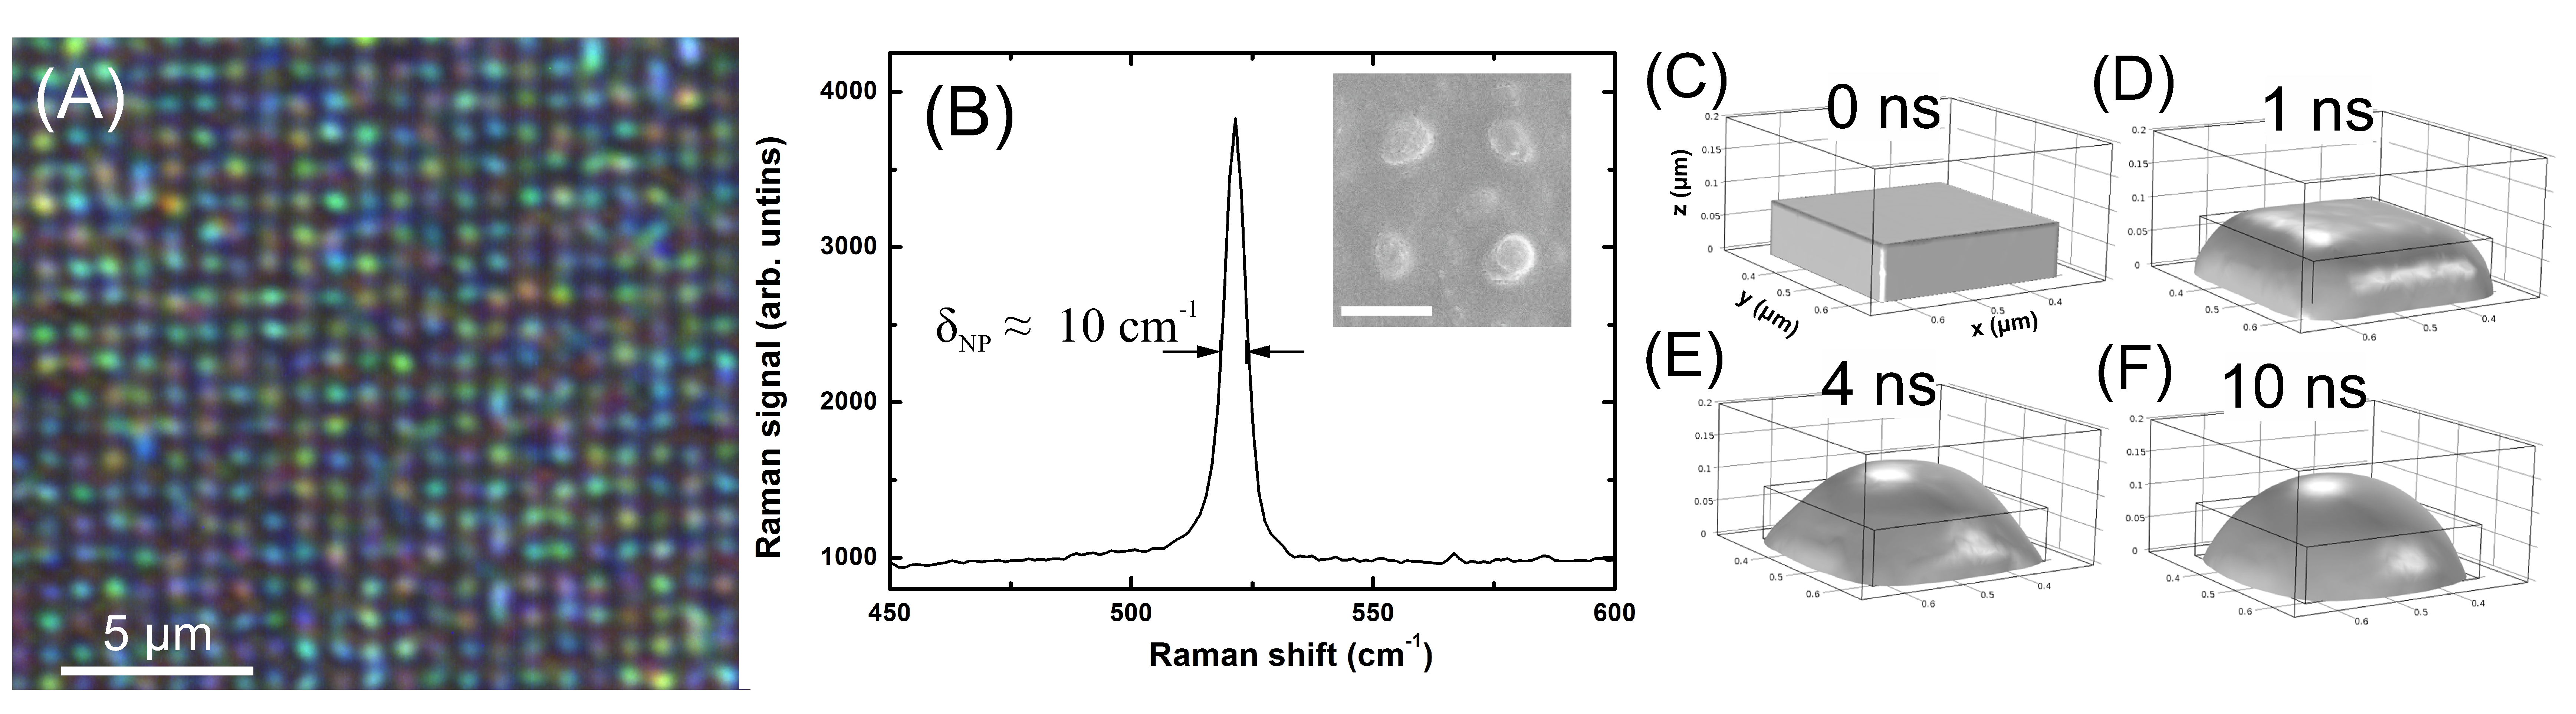
\includegraphics[width=0.9\textwidth]{figs/results/fab/LaserWriting.eps}
                    \end{center}
                    \caption{}
                    \label{fig:LaserWriting}
            \end{figure}

                Under the optimal conditions of fabrication, the method described in Sec.~\ref{met:writing}
            can create and ordered array of nanoparticles, with a period of 0.9~$\mu$m. Dark field imaging of the arrays show that
            the nanoparticles exhibit bright colors, which indicates resonant scattering~--- see Fig.~\ref{fig:LaserWriting}A.
            The cutting process produces square patches, but the resulting arrays are arrays of nearly circular nanoparticles, as can be
            seen on SEM images~--- see Fig.~\ref{fig:LaserWriting}B. This is caused by the dewetting of the thermally isolated patches into
            hemispherical particles, caused be heat accumulation and overheating during the cutting process. COMSOL Simulations of a
            square liquid silicon patch with a side of 300~nm and height of 80~nm on a substrate of fused silica, solving the incompressible
            Navier-Stokes equations with realistic models of the materials show, that after about ten nanoseconds, the the initial patch has
            transformed into an hemisphere with an approximate height and width of 140~nm and 350~nm~--- see Figs.~\ref{fig:LaserWriting}C-F.
            This is in good qualitative agreement with the experimentally observed nanoparticles.

                Measurement of Raman signals from these nanoparticles shows that the particles are, indeed, crystalline~---  they demonstrate
            a narrow peak at 520~cm$^{-1}$, with a half-width of about 10~cm$^{-1}$ (Fig.~\ref{fig:LaserWriting}B).
            This half-width correspond to average crystallite sizes of less than 10~nm, according to previous studies~\cite{campbell1986effects}.

        \subsubsection{Laser Transfer of Nanoparticles}
            \begin{figure}[!ht]
                    \begin{center}
                        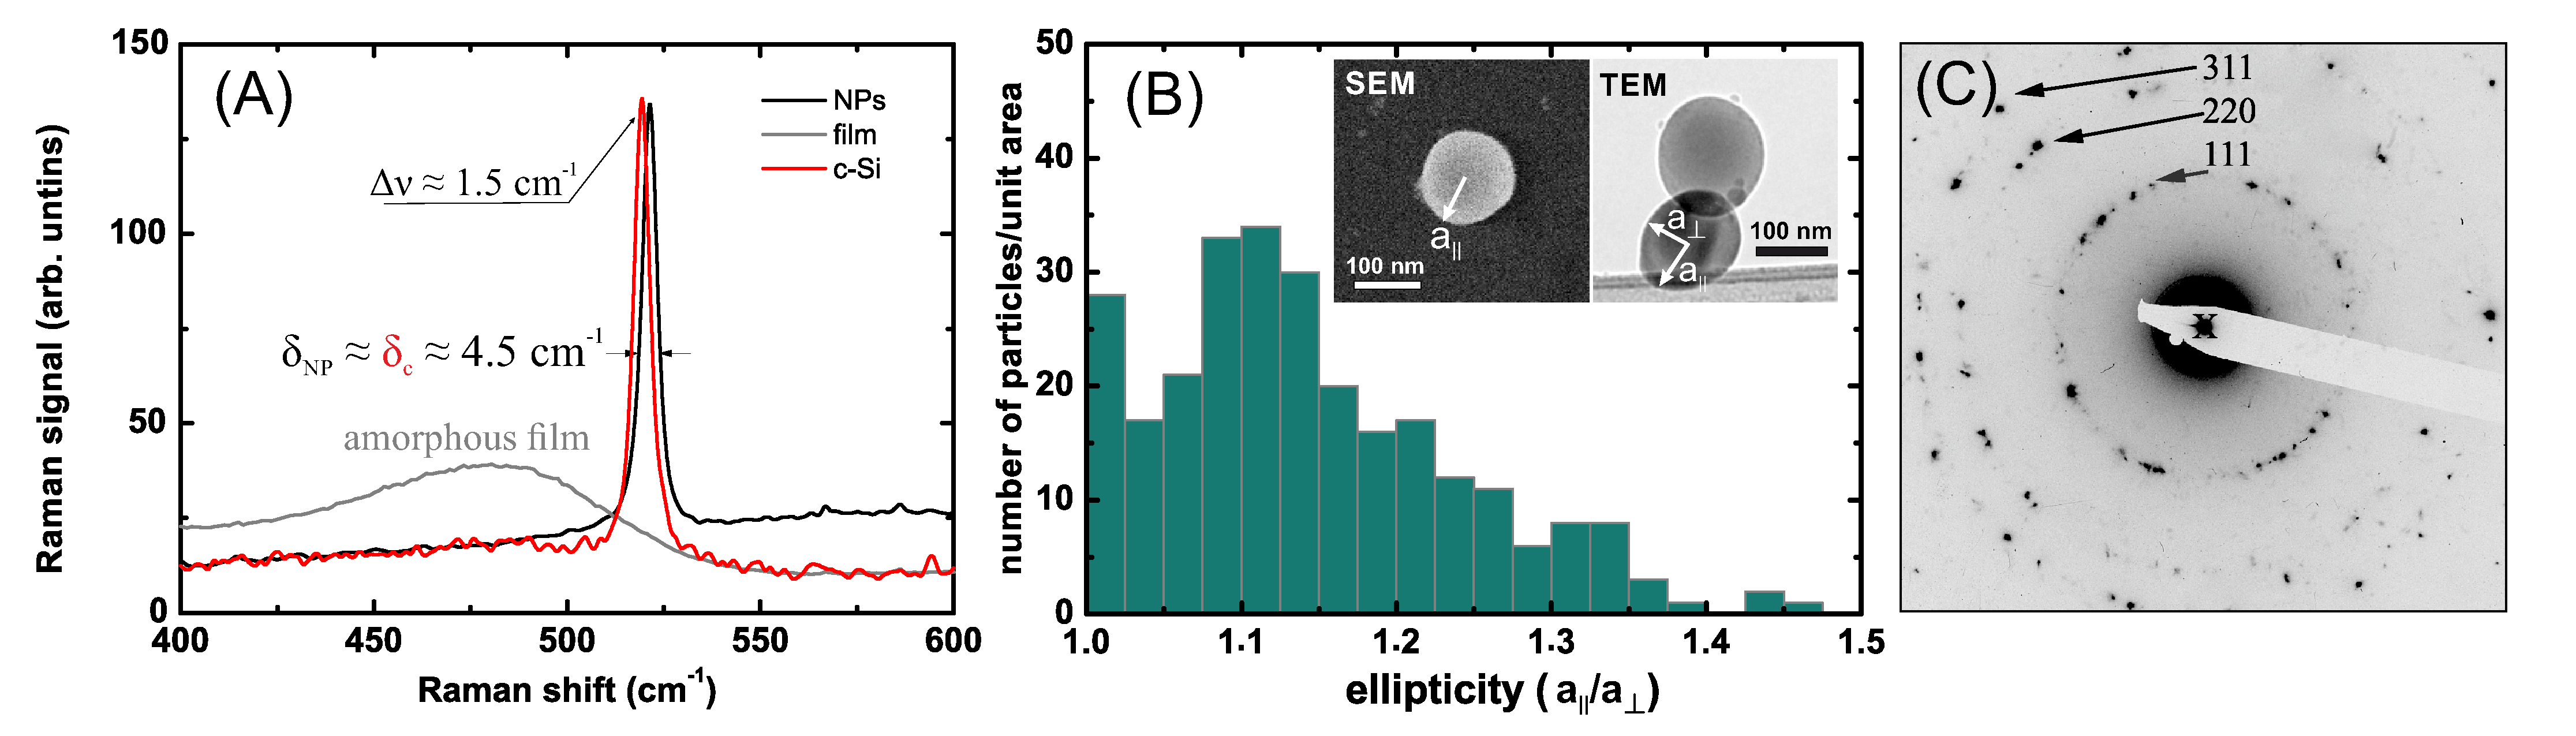
\includegraphics[width=0.9\textwidth]{figs/results/fab/Crystallinity.eps}
                    \end{center}
                    \caption{}
                    \label{fig:Crystallinity}
            \end{figure}


                The initial a-Si:H film, used for the fabrication of the nanoparticles was amorphous, a fact supported by its broad Raman peak,
            centered at 480~cm$^{-1}$. In contrast to the Raman signal of the initial film, the Raman signal from the individual nanoparticles,
            fabricated using the laser transfer method described in Sec.~\ref{met:transfer}, had narrow peaks centered at 521.5~cm$^{-1}$, which
            is very close to the reference Raman signal from a bulk crystalline silicon wafer, centered at 520~cm$^{-1}$. The slight positive shift
            of the position of the Raman peak from the nanoparticles, $\Delta$$\nu$ = 1.5~cm$^{-1}$, can be explained by residual compressive stress
            ~\cite{de1996micro} in the nanoparticles, from the transfer process from donor to acceptor substrate. Similar to the previous method,
            by measuring the half-width of the Raman peak of the nanoparticles, around 4--5~cm$^{-1}$, one can estimate the minimum crystallite size,
            which, in this case is larger than $\sim$20~nm, because the Raman peaks of the nanoparticles have
            almost the same half-width as the peak from a bulk crystalline silicon wafer (4.5~cm$^{-1}$) ~\cite{campbell1986effects}.

                The Raman measurements are supported with electron diffraction patterns of clusters of the printed nanoparticles. The fabricated nanoparticles
            were deposited on transmission electron microscopy specimen grids (3-mm-diameter, 200-mesh copper grids, coated on one side with a 20-nm-thick
            film of amorphous carbon). Using TEM, along with electron diffraction to demonstrate the crystallinity, the size and shape and composition
            of the nanoparticles were studied, using bright and dark field TEM imaging, see Fig.~\ref{fig:Crystallinity}B.
                The electron diffraction pattern from a cluster of nanoparticles shows a number of clear maxima, which correspond to several crystalline planes
            if silicon (Fig.~\ref{fig:Crystallinity}C). Because the specimen grids were even, the particles were deposited at different angles to the substrate,
            allowing their shapes to be studied from the TEM images~--- providing information on the particles' oblateness. The average ellipticity
            of the particles, $a_{\parallel}/a_{\perp}\approx$1.12, where $a_{\parallel}$($a_{\perp}$) is the particle semi-major
            (semi-minor) axis oriented parallel (perpendicular) to the surface of the substrate. Scanning electron microscopy, (SEM, using a Carl Zeiss Neon 40),
            of particles deposited on an flat, even substrate, confirm that the particles possess axial symmetry along the substrate
            normal (Fig.~\ref{fig:Crystallinity}B). These results correlate with previously observed ellipticity of the printed silicon
            nanoparticles~\cite{zywietz2014laser}.

                Previous studies of femtosecond laser ablation as a method of fabricating silicon nanoparticles~\cite{zywietz2014laser, zywietz2014generation}
            have shown that the average size of the fabricated nanoparticles is determined by the laser fluence used. Experiments carried
            out as part of this thesis also showed similar behavior. The experiments demonstrated two distinct regimes of nanoparticle
            fabrication. The first regime, observed at fluencies of up to 150~mJ/cm$^{2}$, has nanoparticle size proportional to the laser
            fluence, which can be seen in Fig.~\ref{fig:Darkfield}A--C as a change in color from blue to red. This can be explained by the
            spallation mechanism of laser ablation, where a thin molten layer is spalled due to the laser-induced tensile pressure waves~\cite{ionin2013thermal,wu2014microscopic},
            breaking into a number of liquid droplets via the Rayleigh-Plateau instability~\cite{papageorgiou1995breakup}.
            The photomechanically spalled volume increases as $V\sim\ln(E)$ when illuminated by a Gaussian beam, because of the
            logarithmic dependence of the spalled surface layer area $r^{2}_{s}\sim\ln(E)$~\cite{bauerle2013laser}, while
            the thickness of the layer remains almost constant~\cite{ionin2013thermal} or even slightly decreases~\cite{wu2014microscopic}.
            Previous studies of nanoparticle fabrication from crystalline silicon an increase of the molten volume led
            to an increase in the number~\cite{zywietz2014generation} and size~\cite{zywietz2014laser}of fabricated nanoparticles,
            which agrees with current results (Fig.~\ref{fig:Darkfield}A--C).

                The second regime of nanoparticle fabrication is observed at fluencies over ~150~mJ/cm$^{2}$, generating large (red) and
            small nanoparticles at the same time, with a broad size distribution~---- see Fig.~\ref{fig:Darkfield}D. This regime is caused
            by the unstable boiling of superheated silicon~\cite{bulgakova2001pulsed, ionin2013thermal, wu2014microscopic}. In this regime,
            nanoparticles are formed by explosive decomposition of material into small droplets and vapor~\cite{itina2009molecular,wu2014microscopic},
            which result in nanoparticles with average sizes less than 100~nm~\cite{amoruso2004generation}. This regime has been extensively
            studied~\cite{amoruso2004generation, tull2006formation} for biomedical applications. The high-fluence regime (Fig.~\ref{fig:Darkfield}D)
            does not produce monodisperse, reproducible nanoparticles, unlike the low low-fluence regimes (Fig.~\ref{fig:Darkfield}A--C). This
            makes the low-fluence regimes more desirable for controllable nanoparticle fabrication and deposition onto acceptor substrates.
            Raman, TEM and SEM characterization of the printed silicon nanoparticles were used to quantify their crystalline phase,
            proving that it is possible to controllably fabricate crystalline silicon nanoparticles from amorphous films with a single stage
            process.

    \subsection{Characterization of Resonant Optical Modes of the Nanoparticles}
        \label{sec:DarkfieldExp}

        \begin{figure}[!ht]
                \begin{center}
                    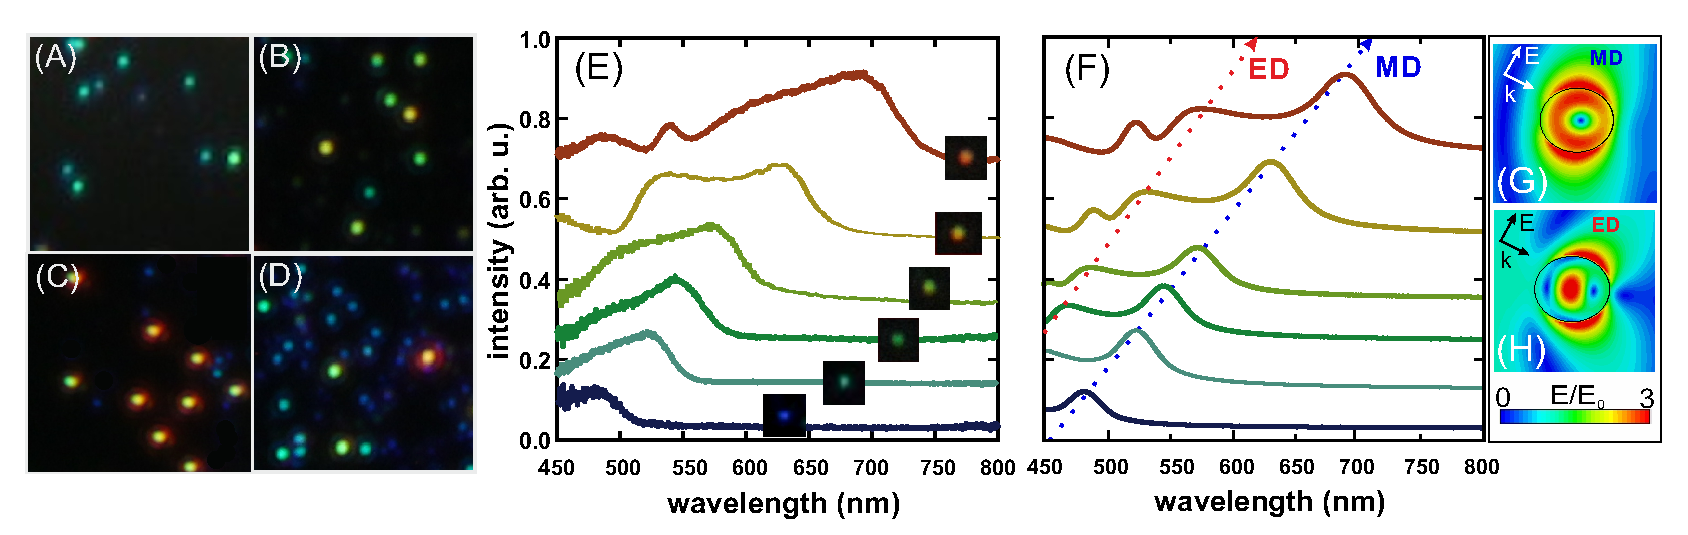
\includegraphics[width=0.9\textwidth]{figs/results/char/DarkField.eps}
                \end{center}
                \caption{Dark-field optical images of silicon nanoparticles fabricated at different peak fluencies:
                120 (A), 130 (B), 140 (C), 160~mJ/cm$^{2}$ (D). Experimental (E) and theoretical (F) spectra for
                scattered p-polarized incident light (angle of incidence is 65$^{\circ}$) from individual nanoparticles
                with the radius parallel to substrate surface a$_{\parallel}$ = 55~nm (blue), 65~nm (spring green),
                68~nm (green), 72~nm (olive), 85~nm (yellow) and 92~nm (red) with the ellipticity coefficient of 1.12.
                Numerically calculated electric field distributions in the silicon nanoparticle with a$_{\perp}$ = 85~nm
                 the wavelengths of 635~nm (G) and 525~nm (H).}
                \label{fig:Darkfield}
        \end{figure}

            Dark field scattering measurements showed that the nanoparticles posses a number of resonances, corresponding to different
        Mie-type resonances, see Fig. \ref{fig:Darkfield}. To determine which resonances correspond to electric dipole (ED) and
        magnetic dipole (MD) resonances, the scattering properties of and electric field distribution near and inside the nanoparticles were
        modeling using the FIT technique in CST Microwave Studio.

            The scattering geometry was modeled as a c-Si ellipsoid with different axis
        ($a_{\perp}$ and $a_{||}$) and the fixed ellipticity $a_{\parallel}/a_{\perp}\approx$~1.12, i.e. for
        the most probable ellipticity parameter in the experiments. The ellipsoid was irradiated by a plane wave
        at the angle 65$^{\circ}$ in vacuum, modeling the geometry used in the dark field scattering experiments. Substrate effects
        were deemed to be insignificant, which is justified in the next section. The optical properties for
        c-Si were taken from Ref.~\cite{vuye1993temperature}. Modeling of scattering spectra (Fig.~\ref{fig:Darkfield}F) showed good agreement
        with the corresponding experimental ones (Fig.~\ref{fig:Darkfield}E), whereas the modeled electric field distributions
        in the ellipsoids at different wavelengths proved the excitation of MD (Fig.~\ref{fig:Darkfield}G) and ED (Fig.~\ref{fig:Darkfield}H).

    \subsection{Determining Size of Nanoparticle from Optical Resonance Positions}

        \begin{figure}[!ht]
                \begin{center}
                    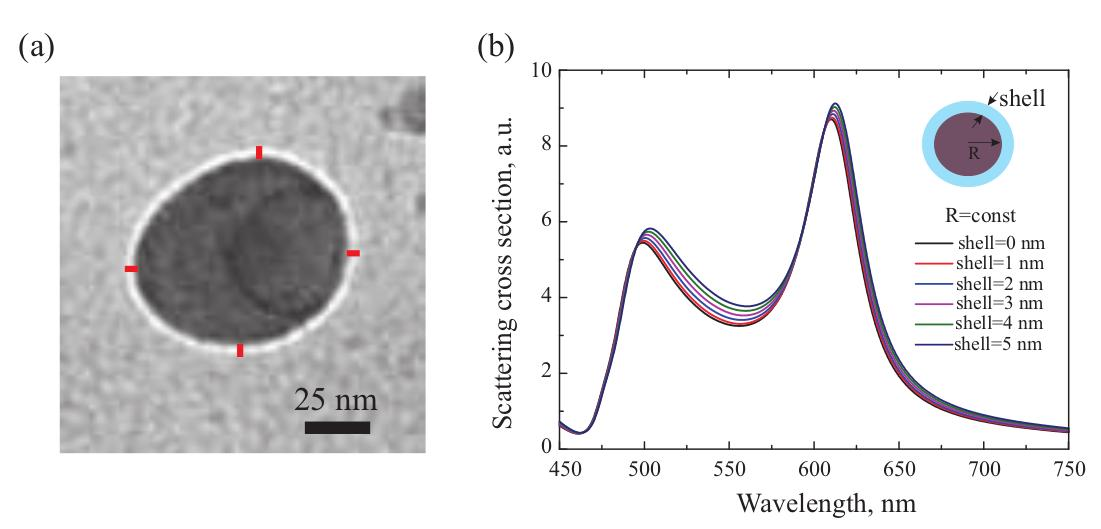
\includegraphics[width=0.9\textwidth]{figs/results/char/CoreShell.jpg}
                \end{center}
                \caption{\textbf{a}. TEM image of the typical silicon nanoparticle fabricated using laser-induced
                            forward transfer technique. Red lines represent 5 nm. \textbf{b}. Total scattering cross sections of
                            silicon nanoparticle (R = 75 nm) coated with silica layers with different thicknesses.}
                \label{fig:CoreShell}
        \end{figure}

        Resonant optical properties of silicon nanoparticles are known to be sensitive to their shape~\cite{zywietz2015electromagnetic},
        crystallinity~\cite{zywietz2015electromagnetic},~\citeA{dmitriev2016laser}, to the substrate~\cite{miroshnichenko2015substrate} and
        to the thickness of native oxide layer~\cite{zywietz2015electromagnetic, fu2012directional},
        which is always present on silicon surface~\cite{morita1990growth}. The shape of the particles was characterized using
        SEM and TEM measurements, while the diameter of silicon core has been extracted from dark-field spectroscopy experiments, by
        comparing the positions of the experimental resonances to those of Mie resonators of different sizes.

        Additional experimental measurements and numerical simulations were done to analyze the influence of native silicon oxide layer
        on the optical properties of the studied nanoparticles. The average thickness of the native oxide layer was
        estimated by transmission electron microscopy (TEM) of a typical silicon nanoparticle, see Fig.~\ref{fig:CoreShell}A.
        The measurements showed that nanoparticles are coated with a thin layer of SiO$_2$, at most 5-nm-thick, which agrees
        with previous results~\cite{zywietz2015electromagnetic, fu2012directional}.
        To analyze the influence of the oxide layer on the resonant properties of nanoparticles,
        total scattering cross section spectra of a crystalline silicon nanoparticle (D = 150 nm) surrounded by
        silica shells with different thicknesses were simulated, see Fig. \ref{fig:CoreShell}. For the sake of simplicity, the simulations have been carried out
        using Mie theory~\cite{bohren1983absorption}. The results of the simulations confirm that in the case of a fixed silicon core diameter, the appearance of an additional
        5-nm-thick silica layer leads to red spectral shifts of both electric and magnetic dipole resonances of the
        nanoparticle at most by $≈ 4.2$nm and $≈ 2.5$nm. The influence of different substrates has been analyzed in
        Ref.~\cite{miroshnichenko2015substrate} The authors have demonstrated that both electric and magnetic dipole resonances of
        crystalline silicon nanoparticle
        placed on the fused silica substrate exhibit small red spectral shifts with respect to the resonances of the nanoparticle
        in free space. In the case of nanoparticle with the diameter of $D = 130 $nm these shifts are around $≈ 3.5 $nm and $≈ 0.5$ nm.
        Therefore, the spectral shift of the nanoparticle’s magnetic dipole resonance is almost insensitive to both
        the substrate and the native silica layer. This allows for accurate estimation of the the diameter of silicon core of the nanoparticle
        from the spectral position of magnetic dipole resonance in the dark-field spectroscopy measurements by
        comparing to the simulations based on Mie theory.


    \subsection{Raman Scattering Enhancement from Single Nanoparticles}
        \label{sec:RamanExp}
        Theoretically predicted enhancement of Raman scattering at different Mie-resonances (see Sec.~\ref{sec:Theory}) was directly compared with to
        experiments with individual crystalline silicon (c-Si) nanoparticles on a fused silica substrate.

        \begin{figure}[!ht]
            \begin{center}
                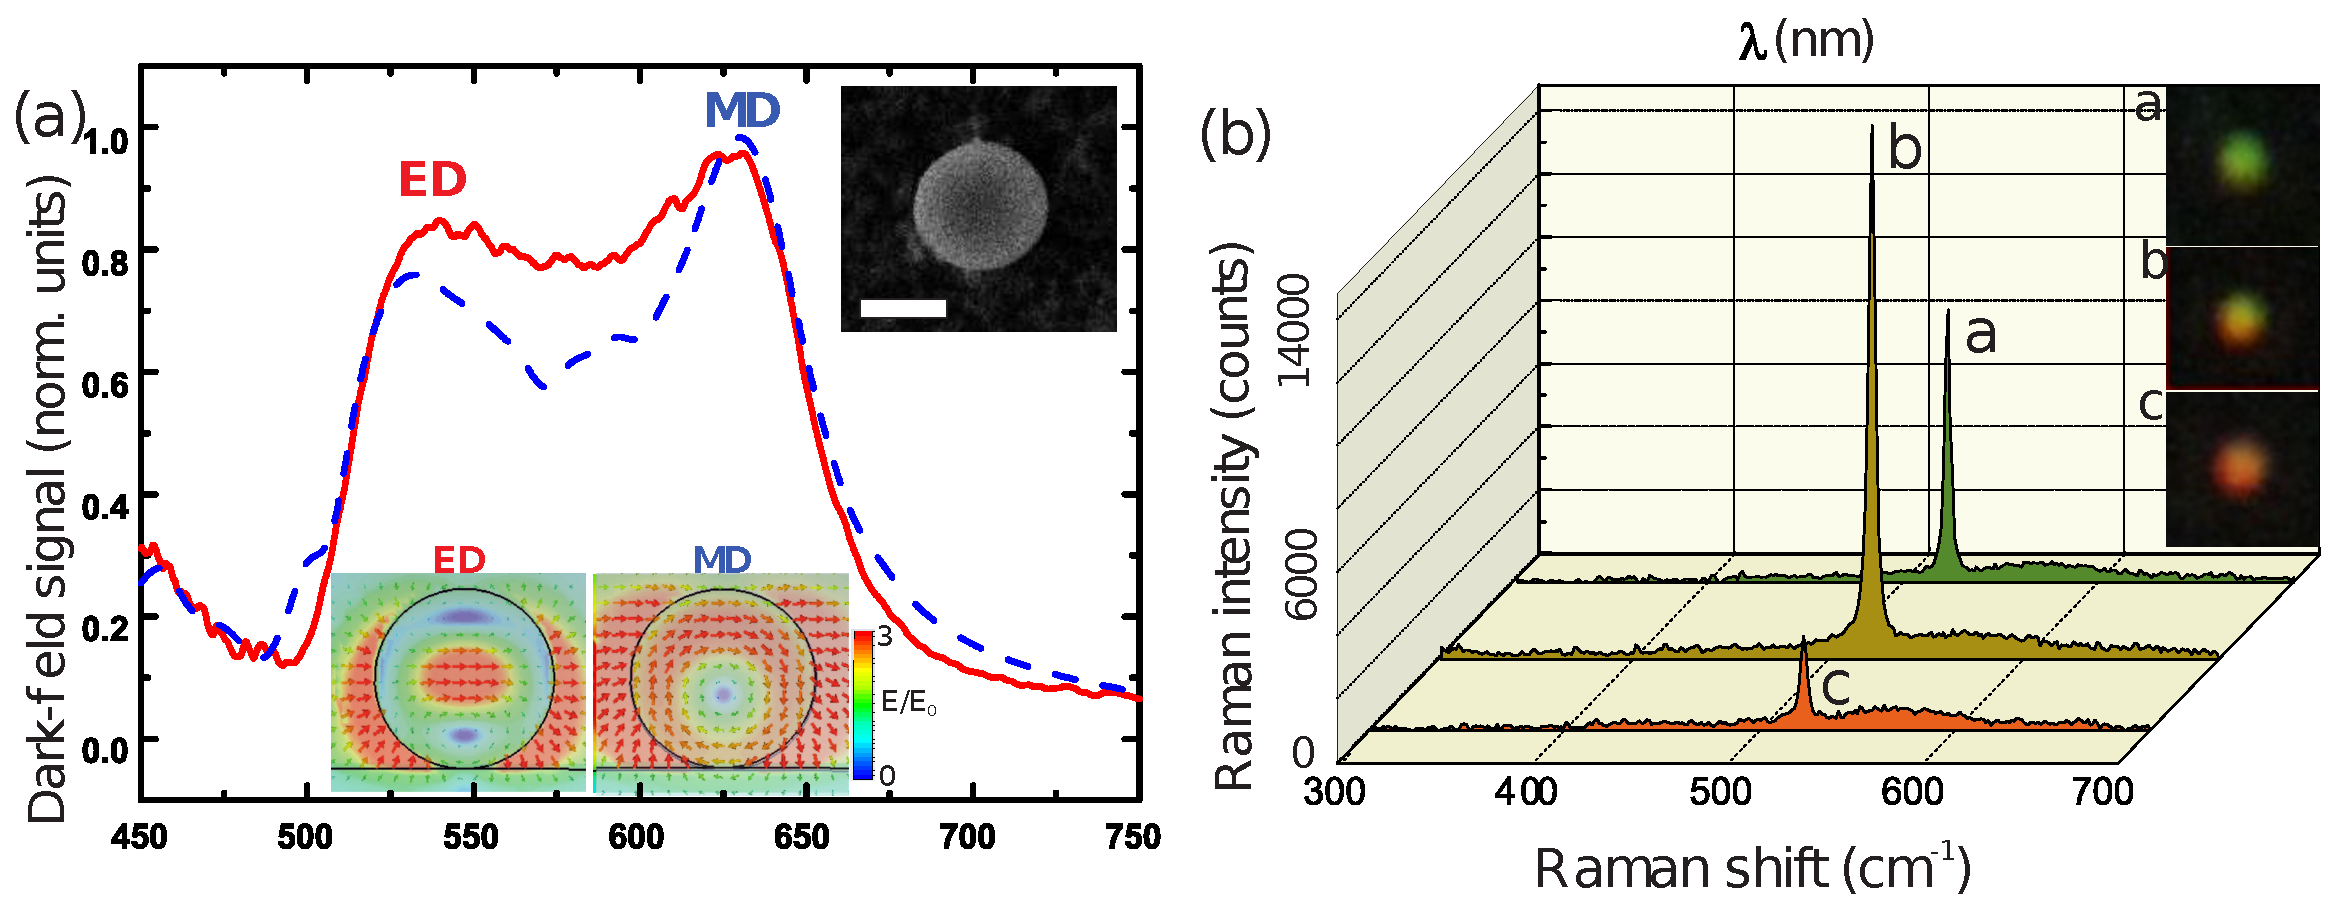
\includegraphics[width=0.9\textwidth]{figs/results/enhance/EnhancementExperiment.eps}
            \end{center}
            \caption{(\textbf{a}) Experimental (solid) and theoretical (dashed) scattering spectra for s-polarized incident light.
            Bottom inset: the electric field distribution at different wavelengths, corresponding to electric dipole (ED) and magnetic
            dipole (MD) resonances. Upper inset: SEM image of typical ablative c-Si nanoparticle (scale bar represents 100~nm). (\textbf{b})
            Raman spectra for different nanoparticles at the excitation wavelength of 633 nm and the corresponding dark-field optical images of the
            nanoparticles: (a) D=153 nm, (b) D=158 nm, (c) D=173 nm.}
            \label{fig:EnhancementExp}
        \end{figure}

        The measured Raman scattering signal from individual nanoparticles exhibits extremely strong dependence on their size
        and color in the dark-field images (Fig.~\ref{fig:EnhancementExp}b). Such a dependence for the excitation light at the wavelength
        $\lambda$=633~nm shows a maximum of Raman scattering for nanoparticles with $D\approx 155$~nm, supporting MD resonance
        at this wavelength. The maximum value of the enhancement factor (EF) for nanoparticles with MD in comparison with
        nanoparticles with diameters $D\approx125$~nm and $D\approx175$~nm is about $EF\approx$140. The calculation of EF
        from experimental data is based on the formula: EF~=~(I/I$_{\rm norm}$)$\times$(V/V$_{\rm norm}$), where I is Raman
        scattering signal from a studied nanoparticle with known diameter and volume V, I$_{\rm norm}$ is Raman signal from
        a nanoparticle of known volume V$_{\rm norm}$ with the smallest observed signal. To make such a normalization, the
        nanoparticle with $D\approx$135~nm was chosen.
        In order to distinguish contributions from each type of Mie resonances, the generalized EF dependence of Raman
        scattering should be represented in terms of the dimensionless nanoparticle diameter $D/\lambda_{\rm Si}$,
        taking into account different refractive indices at different wavelengths (Fig.~\ref{fig:EnhancementExpTheory}). Such a dependence
        exhibits a pronounced maximum with a peak $EF\approx$140 at D/$\lambda_{\rm Si}$ $\approx$ 1, i.e. near the
        magnetic dipole resonance. This value is 5-7 times larger than EF for the electric dipole. Insets in Fig.~\ref{fig:EnhancementExp}a
        provide an illustrative interpretation of this enhancement. At the MD resonance, a larger fraction of electromagnetic
        energy is stored inside the nanoparticle, thus increasing total Raman polarization and emission.
        Corresponding theoretical calculations for perfect spherical c-Si nanoparticles predict even larger difference between
        MD and ED ($\sim$ 10), which is not perfectly matched with the observed results owing to the existence of nanoscale
        deviations and a thin natural oxide layer~\cite{fu2012directional, zywietz2015electromagnetic}. Nevertheless, the
        Raman signal enhancement in the vicinity of MD is in excellent agreement with the analytical model from Sec. \ref{sec:Theory}.
        The data shown in Fig.~\ref{fig:EnhancementExpTheory} is limited to nanoparticle diameters $D/\lambda_{\rm Si}<1.3$ as the fabrication method
        does not allow to make larger particles without pronounced ellipticity. At the same time, even small deviation from the spherical shape leads to
        suppression of the MQ resonance~\cite{fu2012directional}, limiting experimental demonstrations of the enhancement to MD and ED resonances.

        \begin{figure}[!hb]
            \begin{center}
                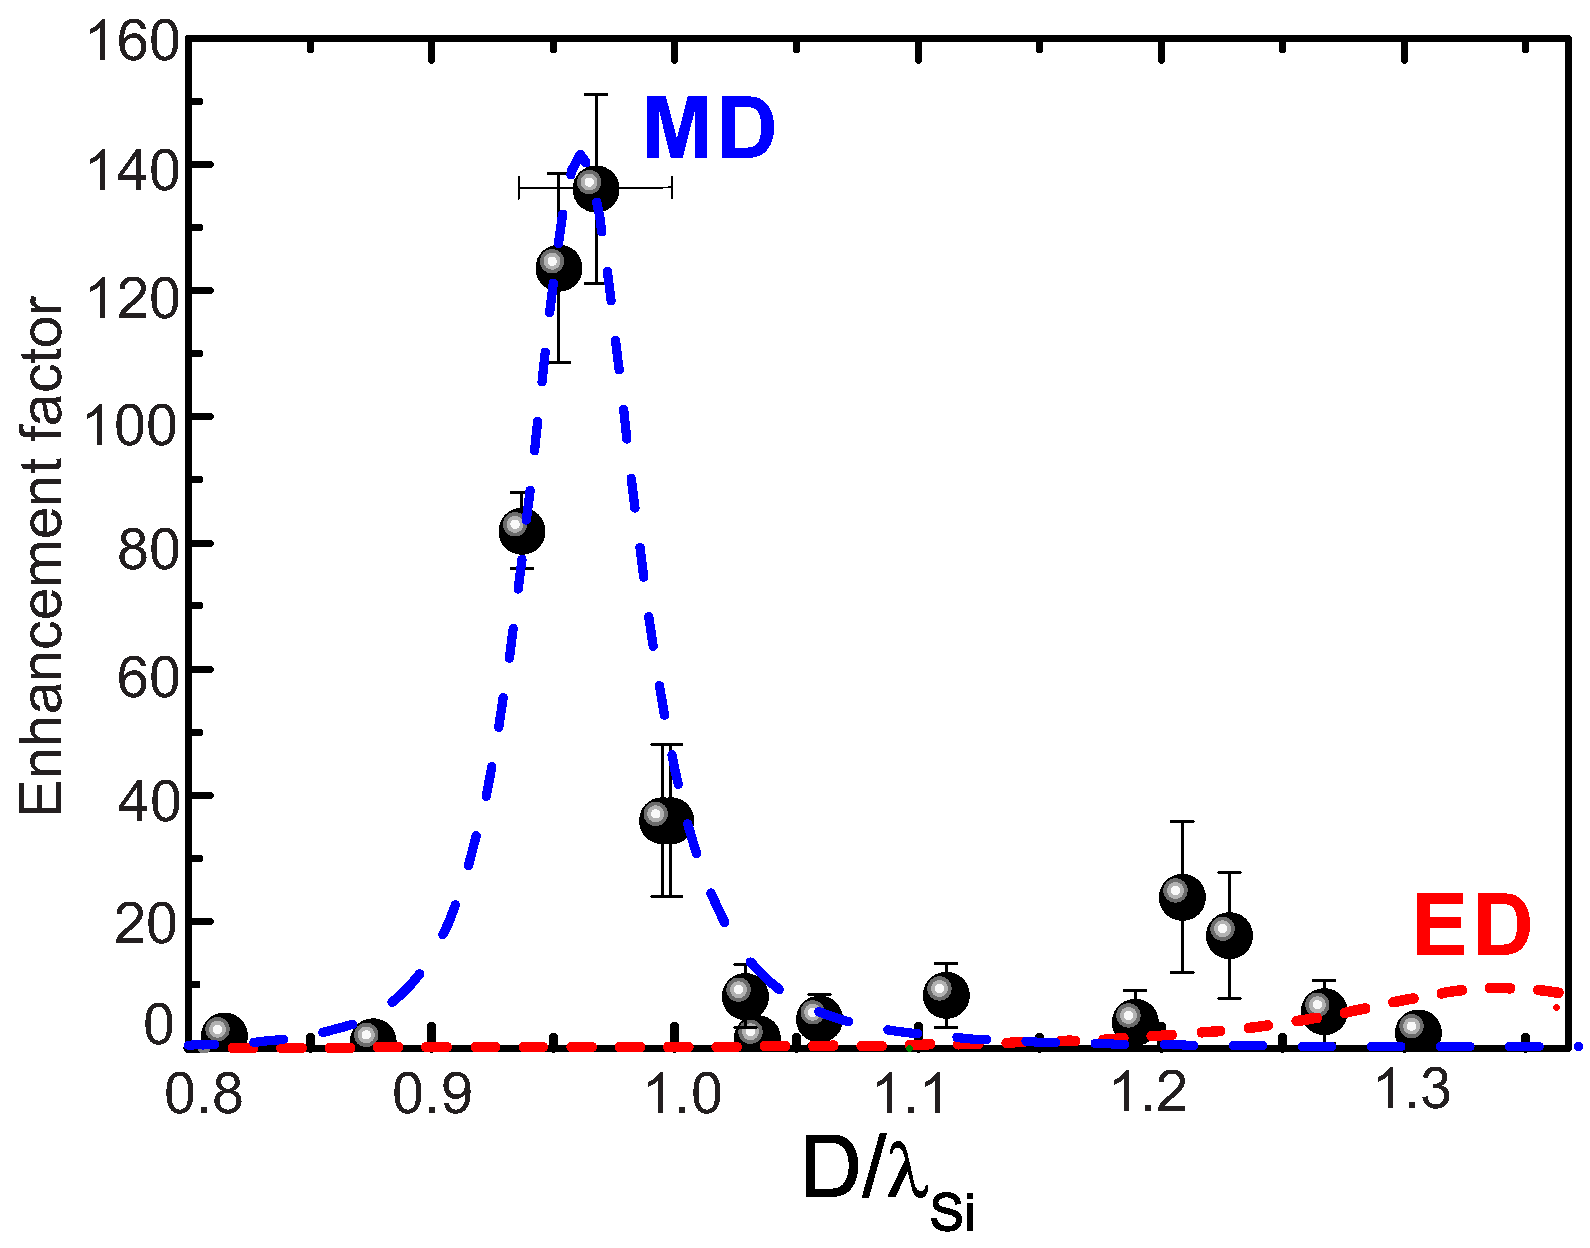
\includegraphics[width=0.5\textwidth]{figs/results/enhance/EnhancementExperimentTheory.eps}
            \end{center}
            \caption{Theoretical (dashed curves) and experimental (black dots) dependencies of the enhancement factor for Raman
            scattering from spherical silicon nanoparticles on their diameter D normalized to the excitation wavelength in silicon.
            Theoretical dependence consists of two contributions from magnetic dipole (blue dashed curve) and electric dipole
            (red dashed curve).}
            \label{fig:EnhancementExpTheory}
        \end{figure}
